\section{Estado del Arte}

Con el objetivo de explorar a fondo el panorama actual de la computación autonómica, y en particular, los mecanismos de adaptación de arquitecturas de software y los requisitos fundamentales para su implementación, se llevó a cabo una revisión de la literatura en diversas bases de datos. Esta revisión abarcó un recorrido que partió de una visión general y se adentró en aspectos cada vez más específicos. Durante este proceso, se examinaron detalladamente las propuestas y componentes clave de sistemas de software autonómicos, así como las diversas nociones relacionadas con notaciones, algoritmos para la comparación de estructuras de datos y los mecanismos esenciales para la adaptación de arquitecturas de software. 

\subsection{Computación Autonómica}

% Definir qué es la computación autonómica y qué es lo que propone

El concepto de computación autonómica, definido inicialmente por IBM \citeyear{horn_2001}, se refiere a un conjunto de características que presenta un sistema computacional el cual le permite actuar de manera autónoma, o auto-gobernarse, con el fin de alcanzar algún objetivo establecido por los administradores del sistema \cite{lalanda_diaconescu_mccann_2014}.


Los 8 elementos clave, definidos por IBM, que deberían presentar este tipo de sistemas son:
% \begin{multicols}{2}
\begin{enumerate}
    \item Auto-conocimiento: habilidad de conocer su estado actual, las interacciones del sistema.
    \item Auto-configuración: capacidad de reconfigurarse frente a los constantes cambios en el entorno.
    \item Auto-optimización: búsqueda constante de optimizar el funcionamiento de sí mismo.
    \item Auto-sanación: aptitud de restaurar el sistema en el caso de que se presenten fallas.
    \item Auto-protección: facultad de protegerse a sí mismo de ataques externos.
    \item Auto-conciencia: posibilidad de conocer el ambiente en el que el sistema se encuentra.
    \item Heterogeneidad: capacidad de interactuar con otros sistemas de manera cooperativa.
    \item Abstracción: ocultar la complejidad a los administradores del sistema con objetivos de alto nivel de abstracción.
\end{enumerate}
% \end{multicols}

En el caso de que un sistema tenga una implementación parcial de estas características, este podría considerarse autonómico. En este sentido debería tener la capacidad de lidiar con los problemas como la complejidad, heterogeneidad e incertidumbre \cite{emerging_2005} al igual que reducir la cantidad de recursos tanto técnicos como humanos requeridos para mantener los sistemas en funcionamiento.

\subsubsection{MAPE-K}

% Explicar como funciona el modelo de management y los pasos que se aplican dentro de lo que se tiene
% Más que todo es desarrollar que es el ciclo MAPE-K

IBM, en cuanto a la implementación de las características, propone una modelo de ciclo auto-adaptativo, denominado MAPE-K \cite{Krikava2013}. Este acercamiento, compuesto de cinco fases, es uno de ciclos de control más usado en implementaciones de sistemas auto-adaptativos y computación autonómica \cite{Arcaini_2015}. En la figura \ref{fig:mapek}, se presentan las fases que \textit{manejador} debe desarrollar para así administrar cada uno de los elementos del sistema computacional basado en una base de conocimiento común \cite{alessandra_2010}. 

\begin{figure}[H]
    \centering
    \caption{El ciclo auto-adaptativo MAPE-K \protect\cite{alessandra_2010}} 
    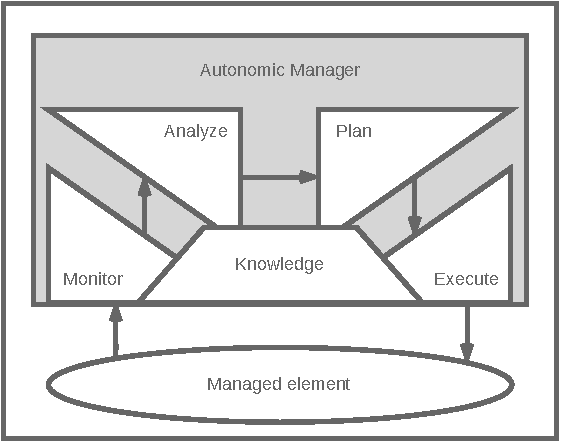
\includegraphics[width=0.8\linewidth]{images/mape-k.pdf}
    \label{fig:mapek}
\end{figure}

Cada una de estas fases son:

\begin{itemize}
    \item Monitorear (M): Esta fase se compone de la recolección, filtración y reportar la información adquirida sobre el estado del elemento a manejar.
    \item Analizar (A): La fase de análisis se encarga del interpretar el entorno en el cual se encuentra, el predecir posibles situaciones comunes y diagnosticar el estado del sistema.
    \item Planear (P): Durante la planificación se determina las acciones a tomar con el fin de llegar a un objetivo establecido a partir de una serie de reglas o estrategias.
    \item Ejecutar (E): Finalmente, se ejecuta lo planeado usando los mecanismos disponibles para el manejo del sistema. 
\end{itemize}

Es de resaltar que este modelo, aunque útil para el desarrollo de este tipo de sistemas, es bastante general en cuanto a la estructura y no usan modelos de diseño establecidos \cite{Ouareth_2018}. 

\subsubsection{Mecanismos de Descripción}

% Esta parte está más que todo para introducir el concepto de la base de conocimiento de la aplicación.
% Es decir, está orientado a dar como un ejemplo de esa base de conocimiento que tiene el "manejador" sobre la 
% plataforma

La fase de monitoreo dentro del ciclo MAPE-K es vital para el funcionamiento del manejador autonómico pues es a partir de la información que se construirá la base de conocimiento requerida por las demás partes del ciclo. Parte de esta, está compuesta por el \textit{estado del sistema} el cual incluye la descripción del sistema en un momento dado \cite{Weiss_2011}.

Existen varias maneras de realizar implementaciones de mecanismos de auto-descripción y la utilidad de cada uno de estos varía dependiendo en el tipo de sistema de software que se esté usando. Para el marco del proyecto, son relevantes aquellas que estén orientados a los sistemas embebidos e  IoT, algunos de estos son:

\begin{itemize}
    \item \textbf{JSON Messaging}: \citeauthor{Iancu_2022} \citeyear{Iancu_2022} plantean un protocolo que emplea mensajería entre \textit{gateways} con el fin de recibir información sobre estas. En términos simples, estas funcionan como un \textit{ping} hacia el nodo que luego retorna sus datos, al igual que los dispositivos conectados a ella, al encargado de recolectar toda esta información con el fin de construir una descripción del sistema.-
    
    \item \textbf{IoT Service Description Model}: O IoT-LMsDM, es un servicio de descripción desarrollado por \citeauthor{Wang_2021} \citeyear{Wang_2021} el cual está orientado al contexto, servicios e interfaz de un sistema IoT. De este se espera poder contar no solo con descripciones del estado del sistema en términos del ambiente, pero la funcionalidad (es decir, los \textit{endpoints} a usar) al igual que las estructuras de datos que estos consumen.
    
    \item \textbf{Adaptadores de Auto-descripción}: En este acercamiento a los mecanismos de auto-descripción, se tienen adaptadores los cuales emplean los datos generados por los sensores del componente gestionado con el fin de realizar la determinación de la arquitectura desplegada. De igual manera, este acercamiento permite realizar modificaciones a la descripción de manera manual en caso de que se detecten problemas \cite{msc_henry_2022}.

\end{itemize}

De esto podemos ver no solo las diferentes maneras en las que las implementaciones realizan las descripciones de los sistemas asociados, sino que también el alcance de estos en cuanto a lo que pueden describir.

\subsubsection{Mecanismos de Adaptación} \label{sec:MecAdap}

% Ya aquí es como definir de manera general qué es eso de los mecanismos de adaptación, qué hacen y qué características
% tienen. 
% No sé si meter ejemplos, creo que eso sería más para un estado del arte en este caso.

La adaptación, en el contexto de la computación autonómica, es la parte más importante en cuanto a la auto-gestión de un sistema de software se refiere. Así mismo, presenta el mayor reto debido a la necesidad de modificar código de bajo nivel, tener que afrontarse a incertidumbre de los efectos que pueden tener dichas alteraciones al sistema al igual que lidiar con esto en \textit{runtime} debido a los problemas que el \textit{downtime} tendría en los negocios \cite{lalanda_diaconescu_mccann_2014}. 

Esta adaptabilidad puede exponerse en múltiples puntos dentro de un sistema de software. Pueden realizarse adaptaciones en sistema operativo, lenguaje de programación, arquitectura e incluso datos \cite{lalanda_diaconescu_mccann_2014}. 

Manteniéndose en el marco del proyecto, son relevantes aquellas soluciones relacionadas con la modificación de la arquitectura. Siendo así, se centraron en los mecanismos de adaptación de componentes, o de reconfiguración:

\begin{itemize}
    \item \textbf{Binding Modification}: Este mecanismo hace referencia a la alteración de los vínculos entre los diferentes componentes de la arquitectura. Estos tienen el objetivo de modificar la interacción entre componentes, lo que es especialmente común en implementaciones con \textit{proxies}. Este tipo de mecanismo de adaptación fue usado por \citeauthor{Kabashkin_2017} \citeyear{Kabashkin_2017} para añadir fiabilidad a la red de comunicación aérea.

    \item \textbf{Interface Modification}: Las interfases funcionan como los puntos de comunicación entre los diferentes componentes de la arquitectura. Siendo así, es posible que la modificación de estos sea de interés con el fin de alterar el comportamiento de un sistema al igual que soportar la heterogeneidad del sistema. Esto puede verse en el trabajo desarrollado por \citeauthor{Liu_2004} \citeyear{Liu_2004} en donde definen la utilidad de dichas adaptaciones al igual que la implementación de las mismas.

    \item \textbf{Component Replacement, Addition and Subtraction}: En términos simples, este mecanismo se encarga de alterar los componentes que componen la arquitectura; de esta manera, modificando su comportamiento. Ejemplos de esto puede verse en el trabajo de \citeauthor{Huynh_2019} \citeyear{Huynh_2019} en el cual se evalúan varios acercamientos a la reconfiguración de arquitecturas a partir del remplazo de componentes a nivel individual al igual que grupal. 
    
    Este acercamiento a la mutación de la arquitectura también puede verse en el despliegue de componentes como respuesta a cambios en los objetivos de negocio de las aplicaciones al igual que como respuesta a cambios inesperados dentro de la aplicación. Esto puede verse en trabajos como el de \citeauthor{Patouni_2006} \citeyear{Patouni_2006} donde se realizan este tipo de implementaciones. 

\end{itemize}

\subsection{Sistemas IoT Autonómicos}

Partiendo de lo anteriormente establecido, una de las áreas en las que estos conceptos de computación autonómica se ha hecho presente es el campo del IoT. Estos acercamientos entre estas dos ramas de las ciencias de la computación se ha venido presentado con la búsqueda de dar a los sistemas IoT la capacidad de adaptarse en a su ambiente con el fin de realizar optimizaciones de los recursos disponibles con el fin de reducir costos, al igual que la necesidad de interacción humana, con la automatización de la configuración así como los procesos de mantener la disponibilidad de los servicios de estos \cite{Ashraf2023}.

Ejemplos de estas implementaciones de propiedades autonómicas en sistemas IoT pueden apreciarse en trabajos como el de \citeauthor{Rajan2011} \citeyear{Rajan2011}, donde después de trabajar con diferentes protocolos de manejo de redes con el fin de poder realizar una administración de una red de sensores, se determinó que el manejo de un sistema de tal magnitud sería la limitante principal en el crecimiento del mismo. Esto terminó en creación de un \textit{control loop} el cual se encargaba de la configuración automática de la red de sensores a partir de parámetros ambientales y objetivos de calidad de servicio.

\subsubsection{Toma de Decisiones en Sistemas IoT Autonómicos}

Algo a resaltar es el tipo de métricas con las cuales se determina la validez. Estas varían dependiendo de las necesidades de las implementación al igual que los objetivos definidos por los administradores del sistema. \citeautoryear{Polanco2023}, identificaron cuatro tipos de maneras de tomar decisiones sobre un sistema IoT.

\begin{itemize}
    \item \textbf{Criterion-Driven}: Orientado principalmente al uso de algoritmos con el fin de establecer el camino a seguir en la toma de decisiones. Este acercamiento puede tener asociado un modelo matemático, algoritmos genéticos, Q-Learning, etc. dependiendo de la complejidad del sistema.
    \item \textbf{Data-Driven}: En este, a partir de datos de entrada y salida definidos, se busca determinar cómo generar datos de nuevo salida definidos dadas unas entradas. Estas están se usan principalmente en implementaciones que usan aprendizaje supervisado o sin supervisión. 
    \item \textbf{Utility-Driven}: En el caso de la utilidad, se refiere a la comparación y evaluación de diferentes alternativas de modelos matemáticos con el fin de establecer una mejor toma de decisiones. Este está relacionado con algunos conceptos usados en teoría de juegos y modelos multicriterio.
    \item \textbf{Probability-Driven}: Este hace uso de modelos probabilísticos, tales como estocásticos o bayesianos, para la toma de decisiones. Normalmente se emplean para aprendizaje no supervisado para la determinación de parámetros a partir de un punto común dados unos datos.
\end{itemize}
